\chapter{Post Processing}
To estimate the magnetic field in Tesla from the flux measurements
(in Webers), the signals must be deconvoluted. The most simple
such deconvolution is simply dividing the flux $\Phi$ by the total surface
area of the coil $A_{coil}$, as in equation \ref{eq:Phi-Area}
\begin{equation}
    \hat{B}[z] = \frac{\Phi[z]}{A_{coil}}
    \label{eq:Phi-Area}
\end{equation}
This gives an estimate $\hat{B}$ of the average $\vb{B}$ field
flowing through the whole coil. The area of the coil can be acquired
either by measuring a known dipole field, or estimated from the
PCB CAD drawings.

Another possibility is fitting the BFF series described in section
\ref{subsec:BFF}, which would give a full three dimensional map of
the whole measurement domain. This is more complicated however,
and requires good modeling of the PCB coils.

\section{Coil Modeling}
\label{sec:coil-modeling}
To fit the BFF series to the flux measurements from the translating
fluxmeter, one needs to take the surface integrals of the coils.
The coil shapes are made up of several spiraling turns, and cannot be
well approximated by simple geometric figures.
Furthermore, the coils span ten layers,
where they start and end at different positions at each layer to make
room for the vias connecting the tracks. Therefore, a python library
was developed to automatically estimate the surfaces from the
PCB CAD files. Each coil first needs to be converted to an
ordered polygon, an ordered set of points defining the path
of the coil.

The CAD files were first converted to KICAD format, an open source
PCB design program. Being open source, the files are easily parsed
since the format is openly available. \cite{noauthor_board_nodate}
Each coil (or net in PCB terms) is then imported, keeping metadata such as
the layer and track width. For each net, there is then an unsorted
array of all the track sections making up the net. Each track
section consists of a start point, an end point and the metadata.
For curved tracks, there is also a mid point. From the three points
a circle can be defined, where a section of the perimeter of the
circle makes up the curved track section. The curved tracks are in the
end discretized as several smaller straight tracks.

Since the tracks are unsorted, and do not necessarily have the
same direction, they need to be sorted. This is done layer by
layer. For each layer, there is an array of $n$ unordered tracks,
with start points $\vb{s_i}$ and end points $\vb{e_i}$.

\begin{equation}
    \begin{pmatrix}
        \vb{s_0} & \vb{e_0} \\
        \vb{s_1} & \vb{e_1} \\
        \vdots   & \vdots   \\
        \vb{s_n} & \vb{e_n} \\
    \end{pmatrix}
\end{equation}

The start and end points are concatenated into one
$n\times 1$ array. To make further equations more clear,
all points will be renamed $\vb{p_i}$
\begin{equation}
    \begin{split}
        &\begin{pmatrix}
            \vb{s_0} &
            \vb{s_1} &
            \cdots   &
            \vb{s_n} &
            \vb{e_0} &
            \vb{e_1} &
            \cdots   &
            \vb{e_n}
        \end{pmatrix}^T = \\
        &\begin{pmatrix}
            \vb{p_0} & \vb{p_1} & \cdots & \vb{p_{2n}}
        \end{pmatrix}^T
    \end{split}
\end{equation}

A distance matrix $M$ of size $2n\times 2n$ is then computed,
containing the pairwise distances of all points.
\begin{equation}
    M =
    \begin{pNiceMatrix}
        \pdist{0}{0}  & \pdist{0}{1}   & \Ldots     & \pdist{0}{2n}    \\
        \pdist{1}{0}  & \Ddots         &            & \Vdots           \\
        \Vdots        &                & \Ddots     & \pdist{2n-1}{2n} \\
        \pdist{2n}{0} & \Ldots         & \pdist{2n}
        {2n-1}        & \pdist{2n}{2n}
    \end{pNiceMatrix}
\end{equation}

Neighboring points are then found by extracting the boolean matrix $N$
from $M$ where the elementwise distances are smaller than some radius $r$.
$r$ is set to be equal to the track width to start, but is iteratively
decreased if the points have more neighbors than expected. This can happen
if the coils contains very short tracks. Each row of $N$ corresponds to
a point, and each column in that row that is equal to 1 corresponds to a
neighbor.

The first $n$ rows in $N$ corresponds to the track
start points, and the last $n$ rows correspond to the track end points.
Then each track segment has its start point neighbors at row $i<n$ and end
point neighbors at row $i+n$. To find the corresponding point $j$ in a track
start/end pair, one simply needs to take the modulus of the row number $i$,
as in equation \ref{eq:trackmodulus}.
\begin{equation}
    j = (i+n)\mod 2n
    \label{eq:trackmodulus}
\end{equation}

Two points on each layer has zero neighbors (exluding the diagonal in
$N$). These are the start and end
points on that layer, connected to a via or a soldering contact on the
first and last layers. Every other point has one neighbor excluding
itself.
The first one of the zero neighbor points is used as a starting point
for the algorithm. Using equation \ref{eq:trackmodulus}, the pair
point for that track segment is found. Continuing, this track segment
will have one neighbor, which is the next point in the polygon. This
continues for all points in the layer, until the other point with no
neighbors is found. For each track segment, one of the start or
end points are discarded, while the other one is put into a polygon
array. This is repeated for each layer in the PCB. The start and end
points for each layer are then matched up to find the orientation
of each polygon array. All layers are then concatenated into one
single polygon array, with the respective layer height added to
each point. The whole coil is now discretely parametrized as an
ordered set of three dimensional points. A plot of one such
set can be seen in figure \ref{fig:pcbpolygon}.

\begin{figure}[!h]
    \centering
    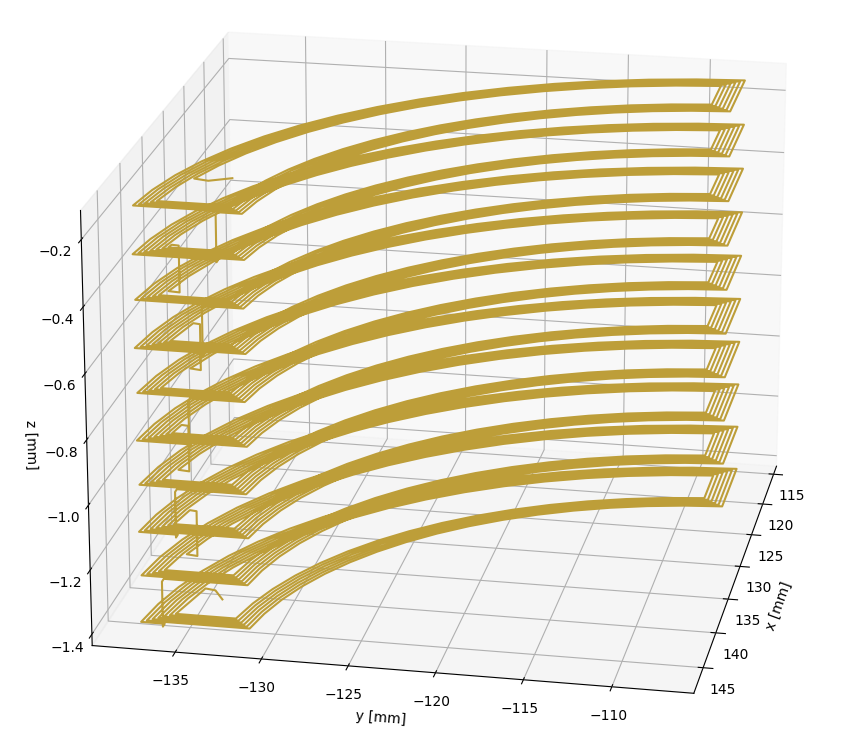
\includegraphics[width=0.8\linewidth]{figs/pcbpolygon}
    \caption{Q31 as an ordered polygon.}
    \label{fig:pcbpolygon}
\end{figure}

With the coils in this polygon format, their total surface area can easily
be approximated using for example the shoelace formula \cite{braden_surveyors_1986}.
This works as a good estimate for the area in equation \ref{eq:Phi-Area}.
For a full deconvolution however, the total surface area is not
enough. The geometric distribution of the surface is also important.

For this purpose, the coil polygons were used to make indicator
functions $\vb{1_A}$. These functions have the property that:
\begin{equation}
    \vb{1_A}(\vb{r}) = \left\{
    \begin{matrix}
        1, & \text{if } \vb{r} \in \vb{A} \\
        0, & \text{otherwise}
    \end{matrix}
    \right.
\end{equation}
where $\vb{A}$ is a surface. The magnetic flux integral of a
coil surface with indicator function $\vb{1_C}$ is then

\begin{equation}
    \Phi(\vb{r}) =
    \int\limits_{-\infty}^{\infty}\int\limits_{-\infty}^{\infty}
    \vb{B}(\vb{r})\vb{1_C}(\vb{r})d\vb{r}
\end{equation}

Several surfaces are estimated for each coil, one for each turn,
on every layer. First, a central point $p_c$ inside the coil is found.
All points on one layer of the coil polygon are converted to
polar coordinates. The central point is then found by taking
the mean of the $r$ and $\varphi$ coordinate. With the central
point found, the coil polygon
$\vb{P} = \left(\vb{p_1}, \vb{p_2} \cdots \vb{p_n} \right)$
is then split into several whole turns using algorithm
\ref{alg:turnsplit}.

\begin{algorithm}
    \caption{Turn-split algorithm for pcb wound coils.}
    \label{alg:turnsplit}
    \begin{algorithmic}
        \State TurnIndices = List()
        \State Turns = 0
        \State angle = 0
        \For{$\vb{p_i} = \left(\vb{p_1}, \vb{p_2} \cdots \vb{p_{n-1}}
                \right)$}
        \State $\vb{v_1} = \vb{p_c} - \vb{p_i}$
        \State $\vb{v_2} = \vb{p_c} - \vb{p_{i+1}}$
        \State angle $+= \vb{v_1}\cdot\vb{v_2}
            /(\|\vb{v_1}\|\|\vb{v_2}\|)$
        \If{angle $>= $Turns$\cdot2\pi$}
        \State \textbf{Append} i to TurnIndices
        \State Turns $+= 1$
        \EndIf
        \EndFor
    \end{algorithmic}
\end{algorithm}

Essentially, for every point in the coil polygon, a two vectors
are drawn from the central point to the current and next point
in $P$. The angle $\varphi$ between these vectors is calculated using their
inner product. This is repeated until the cumulative angle is more
than $2\pi$ times the currently reached number of turns. The indice
of every full turn is saved to a list. This algorithm is also illustrated
in figure \ref{fig:Q11-winding}.

\begin{figure}[!h]
    \centering
    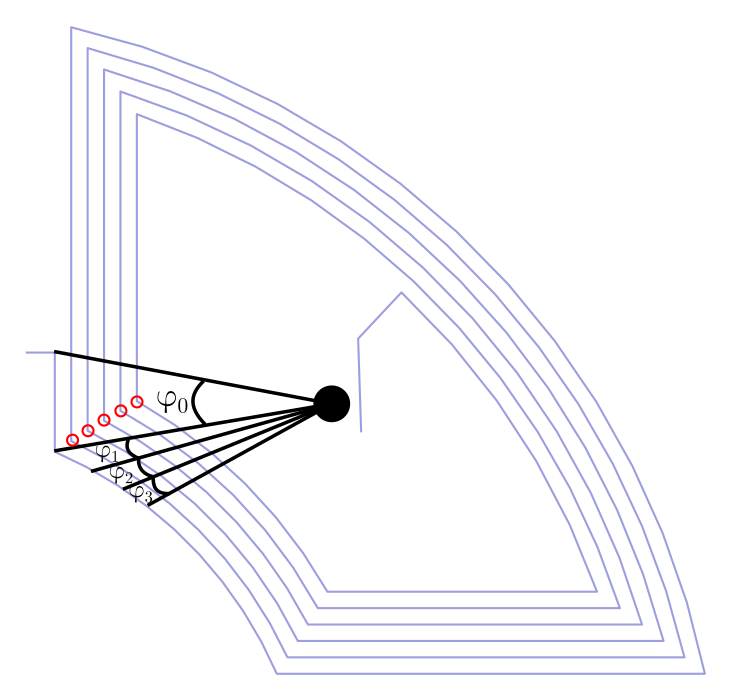
\includegraphics[width=0.8\linewidth]{figs/Q11-roundwalk}
    \caption{Q11 coil winding, with the central point, some
        partial angles, and the estimated whole turns in red.
        Note that curved segments are discretized into smaller
        straight segments.}
    \label{fig:Q11-winding}
\end{figure}

Once the indices for all turns have been found, the polygon is
split into several polygons, one for each turn. The turn polygons
are closed by making them start and end at the same point. Each
coil now has a total amount of turns times layers polygon surfaces.
Two such surfaces can be seen in figure \ref{fig:coilsurfaces}.
In practice, every turn surface is the union of all that turns
surfaces across the layers, to save on expensive surface
integral computations. This slightly
overestimates the amount of surface, but also "smooths" over
the irregularities from the vias and irregular start/end points
across the layers. The surface integrals then only need to
computed once for each turn, and then the results multiplied
by the number of layers.

\begin{figure}[!h]
    \centering
    \begin{subfigure}[b]{0.4\textwidth}
        \centering
        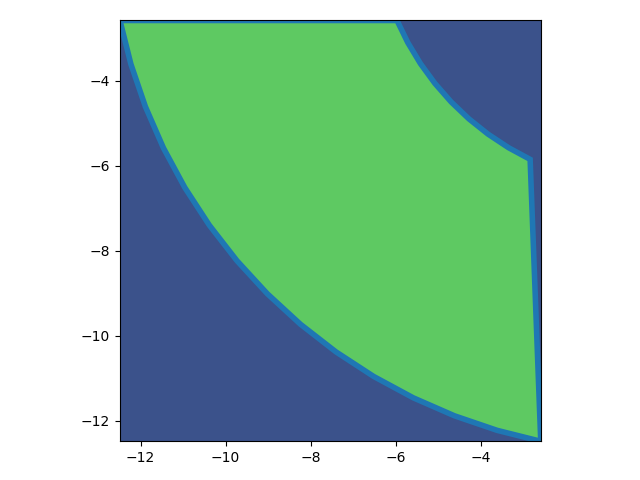
\includegraphics[height=100pt]{figs/Q11-layer0}
        \caption{$Q_{3,1}$ outermost turn surface estimation.}
    \end{subfigure}
    \hfill
    \begin{subfigure}[b]{0.4\textwidth}
        \centering
        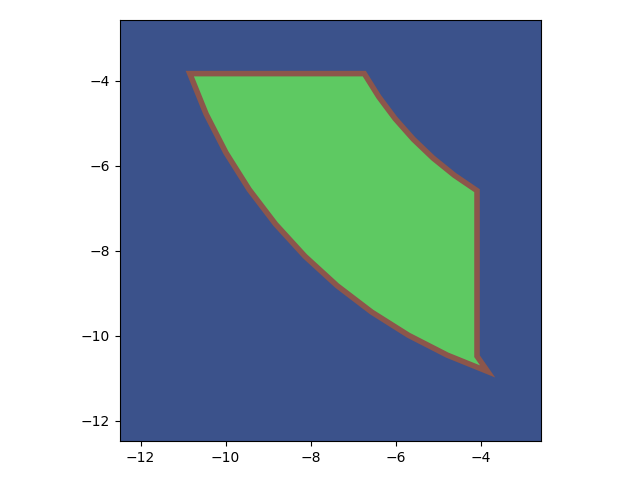
\includegraphics[height=100pt]{figs/Q11-layer5}
        \caption{$Q_{3,1}$ innermost turn surface estimation.}
    \end{subfigure}
    \caption{Estimated coil surface polygons.}
    \label{fig:coilsurfaces}
\end{figure}

The PCB coils have 10 layers with 7 turns per layer. Thus, every
coil produces 7 indicator functions, one for every turn.


\section{Coil Deconvolution and Sensitivity}
\label{sec:coil-deconvolution}
With a way to compute the flux integrals of the coils, the
magnetic flux density can now be properly deconvoluted
from the flux measurements. The flux integral for a
coil can be rewritten in terms of the BFF series.
Since the coils are translated through the magnet
with their normal vector parallel to the $z$ axis, the estimated
flux integral $\hat{\Phi}_C$
for a coil $C$ with surface $A_C$ becomes

\begin{equation}
    \begin{split}
        \hat{\Phi}_C[z_i] &=
        \iint\limits_{A_C}
        \sum\limits_{n=-\infty}^{\infty}
        \sum\limits_{k=-\infty}^{\infty}
        \frac{\partial \Psi_{n,k}}{\partial z}
        (r,\varphi, z|z=z_i) dA \\
        &= \sum\limits_{n=-\infty}^{\infty}
        \sum\limits_{k=-\infty}^{\infty}
        \iint\limits_{A_C}
        \frac{\partial \Psi_{n,k}}{\partial z}
        (r,\varphi, z|z=z_i)dA
    \end{split}
\end{equation}

Let $\psi_{n,k} = \Psi_{n,k}/\Cnk[n,k]$. Since $\Cnk[n,k]$ are
constants, they can be moved out of the integral.

\begin{equation}
    \hat{\Phi}_C[z_i]
    = \sum\limits_{n=-\infty}^{\infty}
    \sum\limits_{k=-\infty}^{\infty}
    \Cnk
    \iint\limits_{A_C}
    \frac{\partial \psi_{n,k}}{\partial z}
    (r,\varphi, z|z=z_i)dA
    \label{eq:psi-integral}
\end{equation}

Let $|n| < N, |k| < K$.
Equation \ref{eq:psi-integral} can now be
written as a matrix equation

\begin{equation}
    \begin{split}
        &\hat{\Phi}_C[z_i] = \\
        &=\iint\limits_{A_C}
        \frac{\partial}{\partial z}
        (\psi_{-N, -K}, \psi_{-N, -K+1}, \ldots,
        \psi_{0, 0}, \ldots, \psi_{N, K-1}, \psi_{N, K})
        dA
        \begin{pmatrix}
            \Cnk[-N, -K] \\ \Cnk[-N, -K+1]\\ \vdots\\
            \Cnk[0, 0]   \\ \vdots \\ \Cnk[N, K-1]\\ \Cnk[N, K]
        \end{pmatrix}
    \end{split}
\end{equation}

Now, denote the leftmost column vector as $\vb{V}_C[z_i]$,
containing the terms of the surface integrals of $\psi_{n,k}$,
with integral surface of coil $C$ at $z$ offset $z_i$. The flux
measurements can now be inserted into the matrix equation, denoting
a measurement sample from coil $C$ at position $z_i$ with $s_C[z_i]$.
This allows us to formulate the measurements and BFF series as
a least squares problem. Let $X$ be the matrix of surface
integrals, $\frak{C}$ the row vector of $\Cnk$ coefficients,
$E$ the row vector of measurement and modeling errors $e[z_i]$, and
$S$ the row vector of measurement samples. The model is then
formulated as $X\frak{C} + E = S$, or more explicitly written
in equation \ref{eq:matrixmodel}.


\begin{equation}
    \begin{pmatrix}
        \vb{V}_C[z_0]     \\ \vb{V}_C[z_{1}] \\ \vdots \\
        \vb{V}_C[z_{i-1}] \\ \vb{V}_C[z_i]
    \end{pmatrix}
    \begin{pmatrix}
        \Cnk[-N, -K] \\ \Cnk[-N, -K+1]\\ \vdots\\
        \Cnk[0, 0]   \\ \vdots \\ \Cnk[N, K-1]\\ \Cnk[N, K]
    \end{pmatrix}
    + \begin{pmatrix}
        e[z_0]     \\ e[z_1]\\ \vdots\\
        e[z_{i-1}] \\ e[z_i]
    \end{pmatrix} =
    \begin{pmatrix}
        s_C[z_0] \\ s_C[z_1] \\ \vdots \\ s_C[z_{i-1}] \\
        s_C[z_i]
    \end{pmatrix}
    \label{eq:matrixmodel}
\end{equation}

The least squares problem is then formulated as finding the
coefficients $\frak{C}$ that minimizes the expression
$\| X\frak{C} - S \|$.
The $\Cnk$ coefficients can now easily be found using a
least squares solver. Furthermore, measurements from
several coils can be added to the equation, allowing one
to fit one model to as many coils as desired.

The $X$ matrix is of particular interest. It contains the
surface integrals of all given coils. This gives a good
indication of the sensitivity of the coils to the different
harmonics in the BFF series. This matrix is visualized in
figure \ref{fig:sensitivity}. Only the coils with unique
geometries are visualized. $Q_{1,4}$ and $Q_{2,4}$ will
for instance have the exact same sensitivity since they
are geometrically identical, save for their rotation and
position on the coil.

\begin{figure}[!h]
    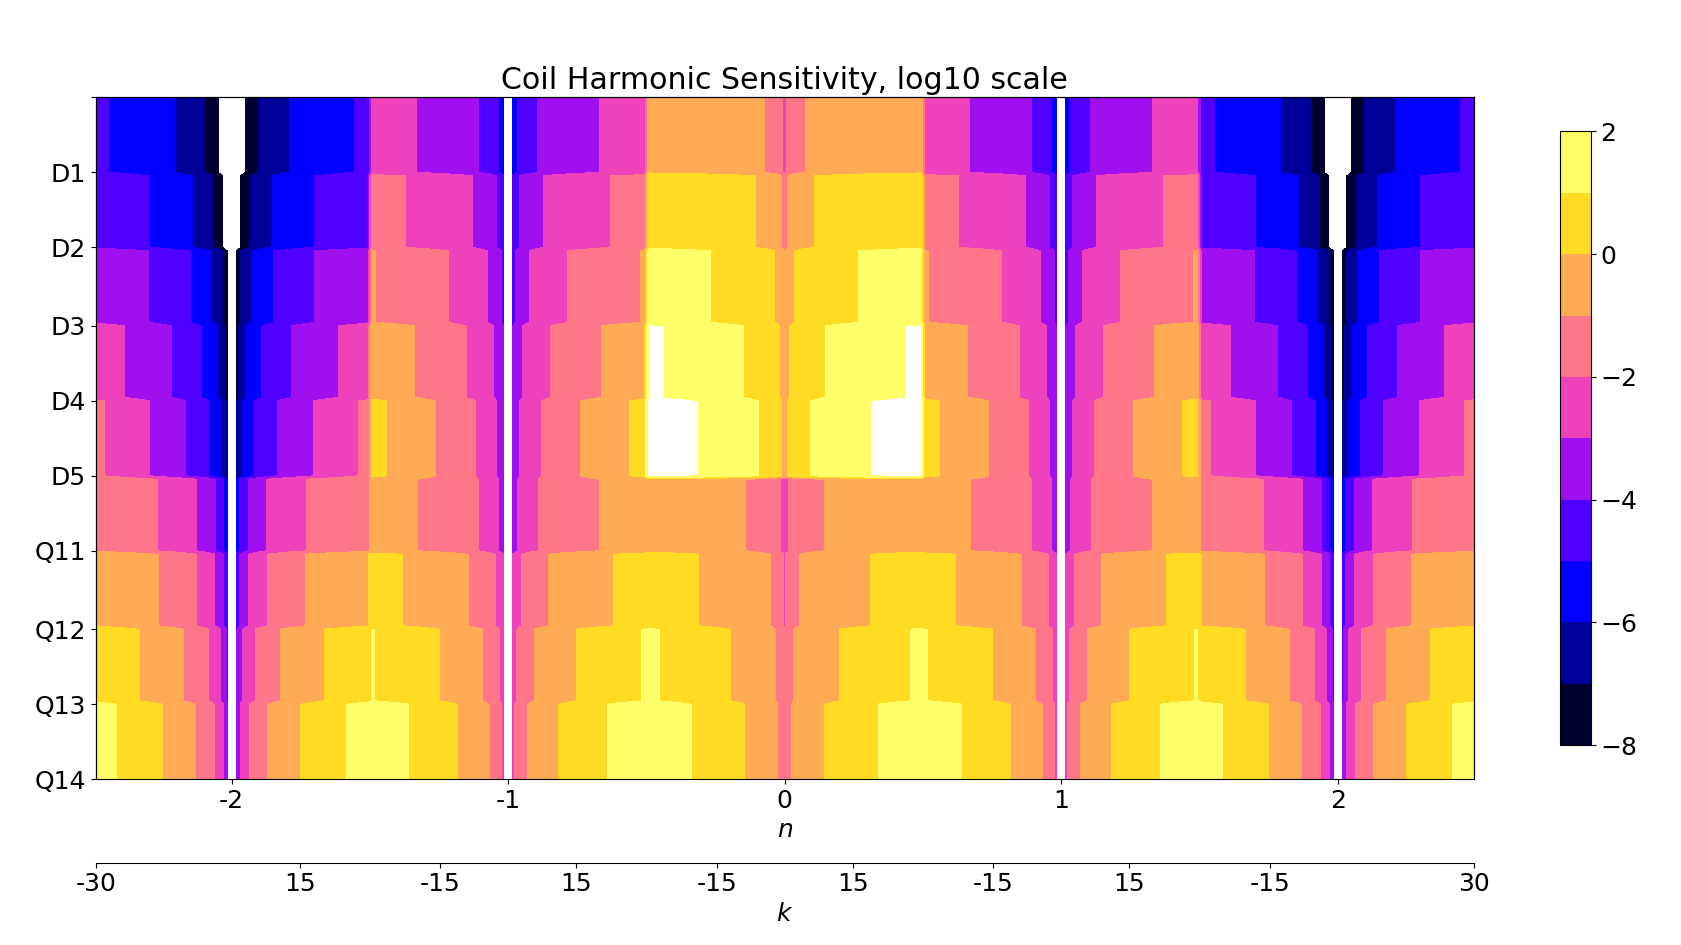
\includegraphics[width=\linewidth]{figs/sensitivity}
    \caption{Sensitivity for the different coils present on
        the fluxmeter.}
    \label{fig:sensitivity}
\end{figure}

Some interesting (and mostly expected) conclusions can be drawn
from figure \ref{fig:sensitivity}. The disc coils are
several orders of magnitude more sensitive to the
solenoid fundamentals than the harmonics, verifying that
they're insensitive to the peak shift from magnet tilt, as
seen in the measurements. The sector coil are on the other
hand relatively much more sensitive to higher orders of both $k$
and $n$, making them a lot more sensitive to the peak shifts.
The disc coils, particularly the largest ones have the largest
sensitivity to any single component, simply because they have more
surface area.
No coils are sensitive to the multipole components. Because
the $B_r$ and $B_\varphi$ components vanish in the flux integrals,
so do the multipole components. This is unfortunate, as it means
that only the $B_z$ field can be fully estimated using this model.

It should be noted that the coil sensitivity is not the only thing
predicting a good fit. One must be mindful of the Nyquist criterium
in all three dimensions. The Bessel-Fourier-Fourier series is
a fourier series in $\varphi$. Therefore, the number of coils
spread out over $\varphi$ puts an upper bound on $n$.
Likewise, the number of samples
along the $z$ axis puts an upper bound on the order of $k$. From
equation \ref{eq:Psi} it can be seen that the geometric frequency
in $z$ $f_z$ can be expressed as
\begin{equation}
    f_z = \frac{2\pi}{L}|k|
    \label{eq:fz}
\end{equation}
and the geometric frequency in $\varphi$
\begin{equation}
    f_{\varphi} = |n|
    \label{eq:fphi}
\end{equation}

\section{Bessel-Fourier-Fourier Series Fitting}
\label{sec:BFF-fitting}
On the fluxmeter, there are four
sector coils per radial layer, giving us four points in $\varphi$.
Using the Nyquist criterion along with equation \ref{eq:fphi}
then gives us the upper bound on fitting in $n$
\begin{equation}
    |n|_{\text{max}} < \frac{4}{2} = 2
\end{equation}

The maximum order of $k$ can be computed in a similar way
using equation \ref{eq:fz}.
The measurements are spaced
along the z axis with a distance of $0.11$ mm, or
$\frac{1}{0.00011} \approx 9090$ samples/m. The fluxmeter
measurements spanned 1.5 meters.
The upper bound on $k$ can then be found
\begin{equation}
    |k|_{\text{max}} < \frac{9090\cdot 1.5}{2\cdot 2\pi} \approx 1085
\end{equation}
When fitting in practice, an order $k=30$ was found to be
more than sufficient for a good fit, and $n$ was chosen to
be equal to 1. Through experimentation, it was also found
that fitting using just the $D_5$ coil and the outermost
sector coils $Q_{1,4}-Q_{4,4}$ was sufficient. A better fit
was not achieved by using more coils. By studying figure
\ref{fig:sensitivity}, one can see that the measurements
from these coils is enough to determine the $\Cnk$
coefficients, or at least that the remaining coils give
little further benefit to the fit. In this section, a
fit of a measurement with a yaw angle of $58$ mrad is
showcased.

The fits are plotted along with their respective measurements
in figures \ref{fig:Dfit}-\ref{fig:Q1fit}. The errors for
some chosen coils can be seen in table \ref{tab:fitting-errors}.

From these results, it can be seen that the
fitting error is generally around the same magnitude, but tends
to be smaller the larger the coil is, both in absolute and
normalized terms. A likely explanation is that for coils
with a smaller surface area, errors in the coil surface
modeling will have a larger impact.

\begin{table}[!h]
    \centering
    \begin{tabular}{l p{2cm} p{2cm} p{2cm} p{2cm}}
            & Mean Error {[}Wb{]} & Max Error {[}Wb{]} & Mean Error Normalized & Max Error Normalized \\ \hline
        D1  & 1.30E-05            & 3.50E-05           & 3.08\%                & 8.30\%               \\
        D2  & 2.07E-05            & 4.17E-05           & 0.73\%                & 1.48\%               \\
        D3  & 1.13E-05            & 2.36E-05           & 0.13\%                & 0.28\%               \\
        D4  & 4.18E-05            & 8.63E-05           & 0.24\%                & 0.50\%               \\
        D5  & 4.84E-06            & 2.93E-05           & 0.02\%                & 0.10\%               \\
        Q11 & 1.08E-05            & 2.57E-05           & 4.98\%                & 11.86\%              \\
        Q12 & 7.26E-06            & 1.48E-05           & 1.23\%                & 2.50\%               \\
        Q13 & 1.61E-06            & 7.56E-06           & 0.17\%                & 0.79\%               \\
        Q14 & 1.39E-06            & 4.30E-06           & 0.10\%                & 0.32\%
    \end{tabular}
    \caption{Fitting errors for selected coils.}
    \label{tab:fitting-errors}
\end{table}

\begin{figure}[!h]
    \centering
    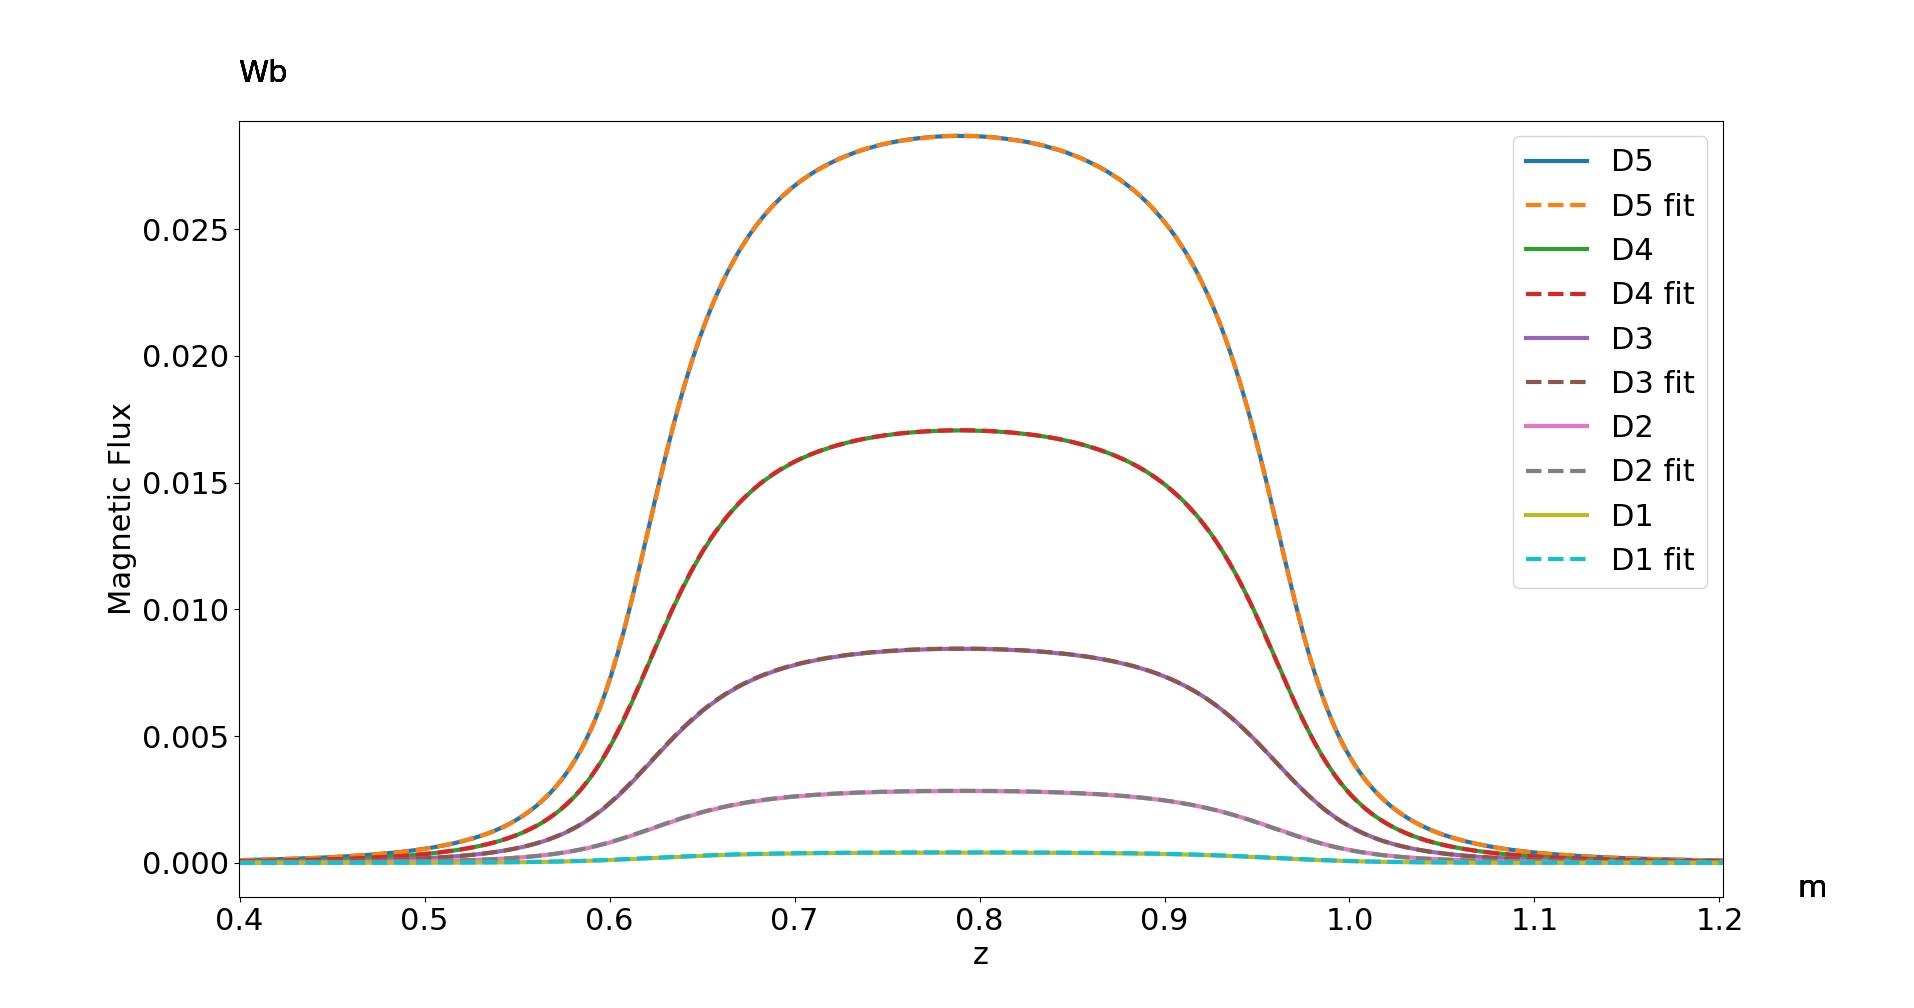
\includegraphics[width=\linewidth]{figs/Dfit}
    \caption{Measurements and BFF fit, $D_l$ coils.}
    \label{fig:Dfit}
\end{figure}

\begin{figure}[!h]
    \centering
    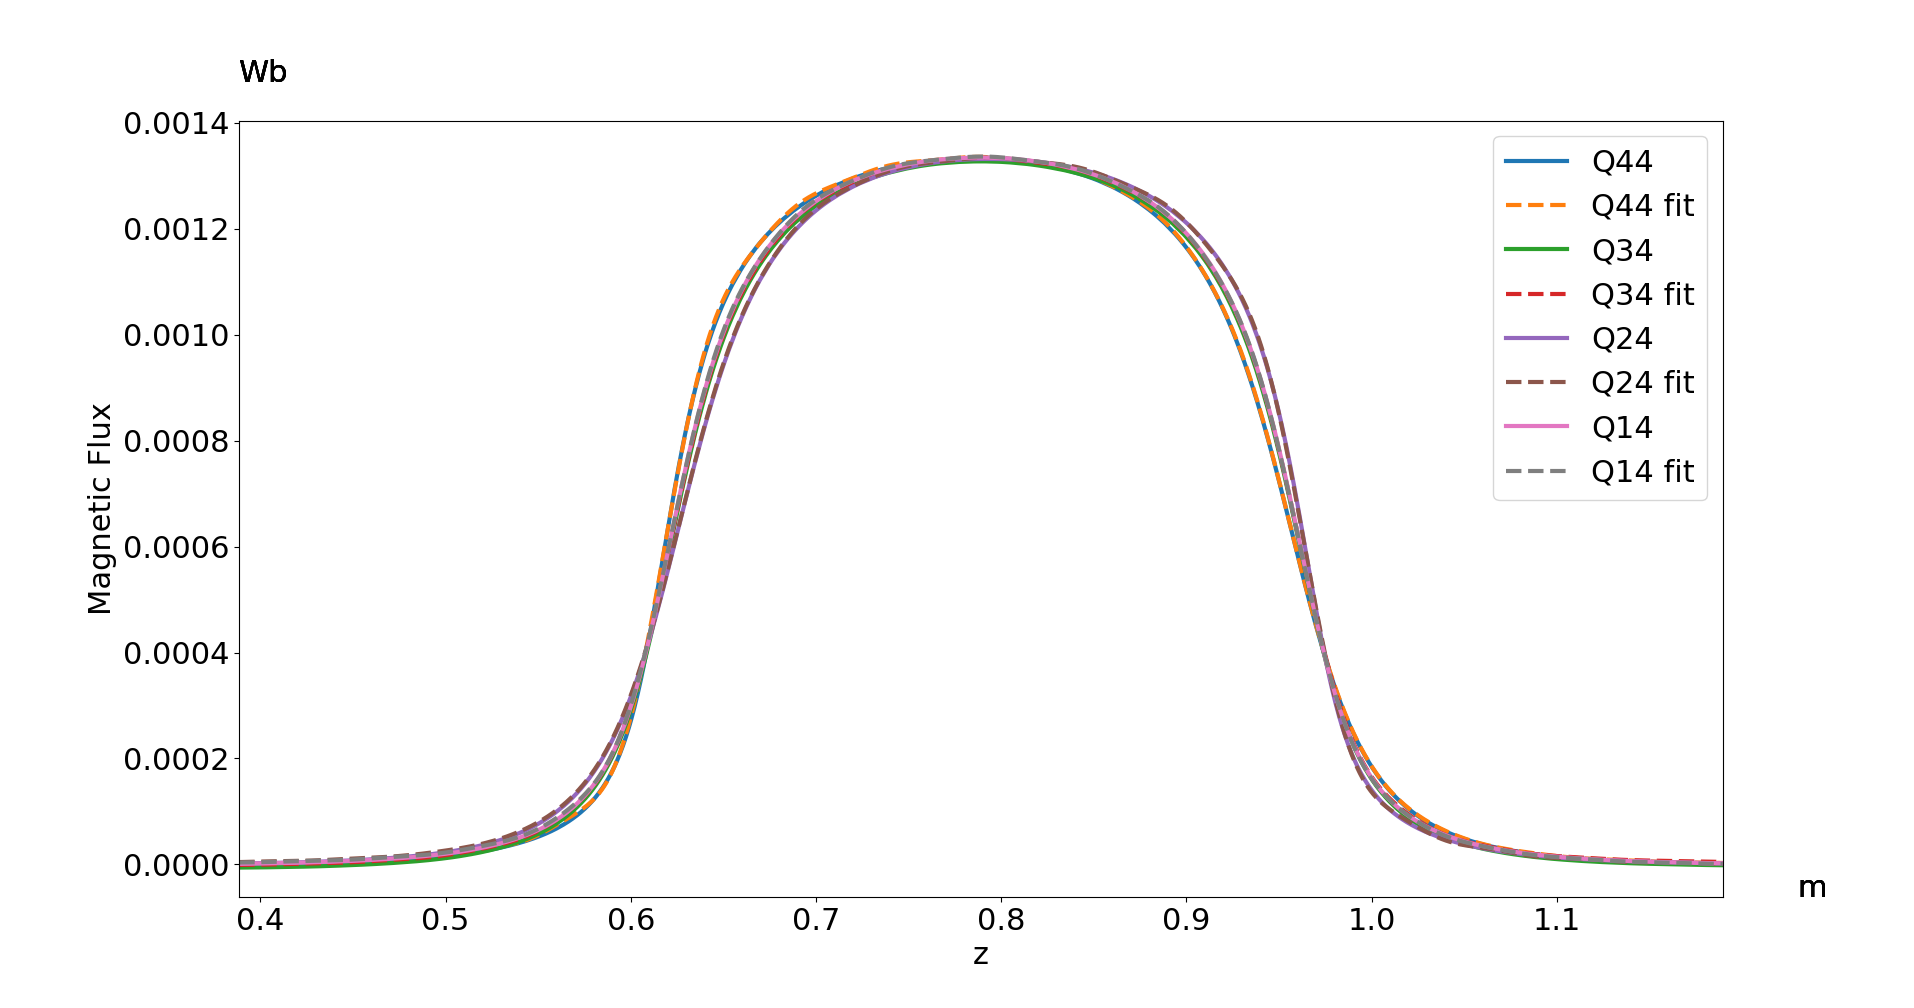
\includegraphics[width=\linewidth]{figs/Q4fit}
    \caption{Measurements and BFF fit, $Q_{q,4}$ coils.}
    \label{fig:Q4fit}
\end{figure}

\begin{figure}[!h]
    \centering
    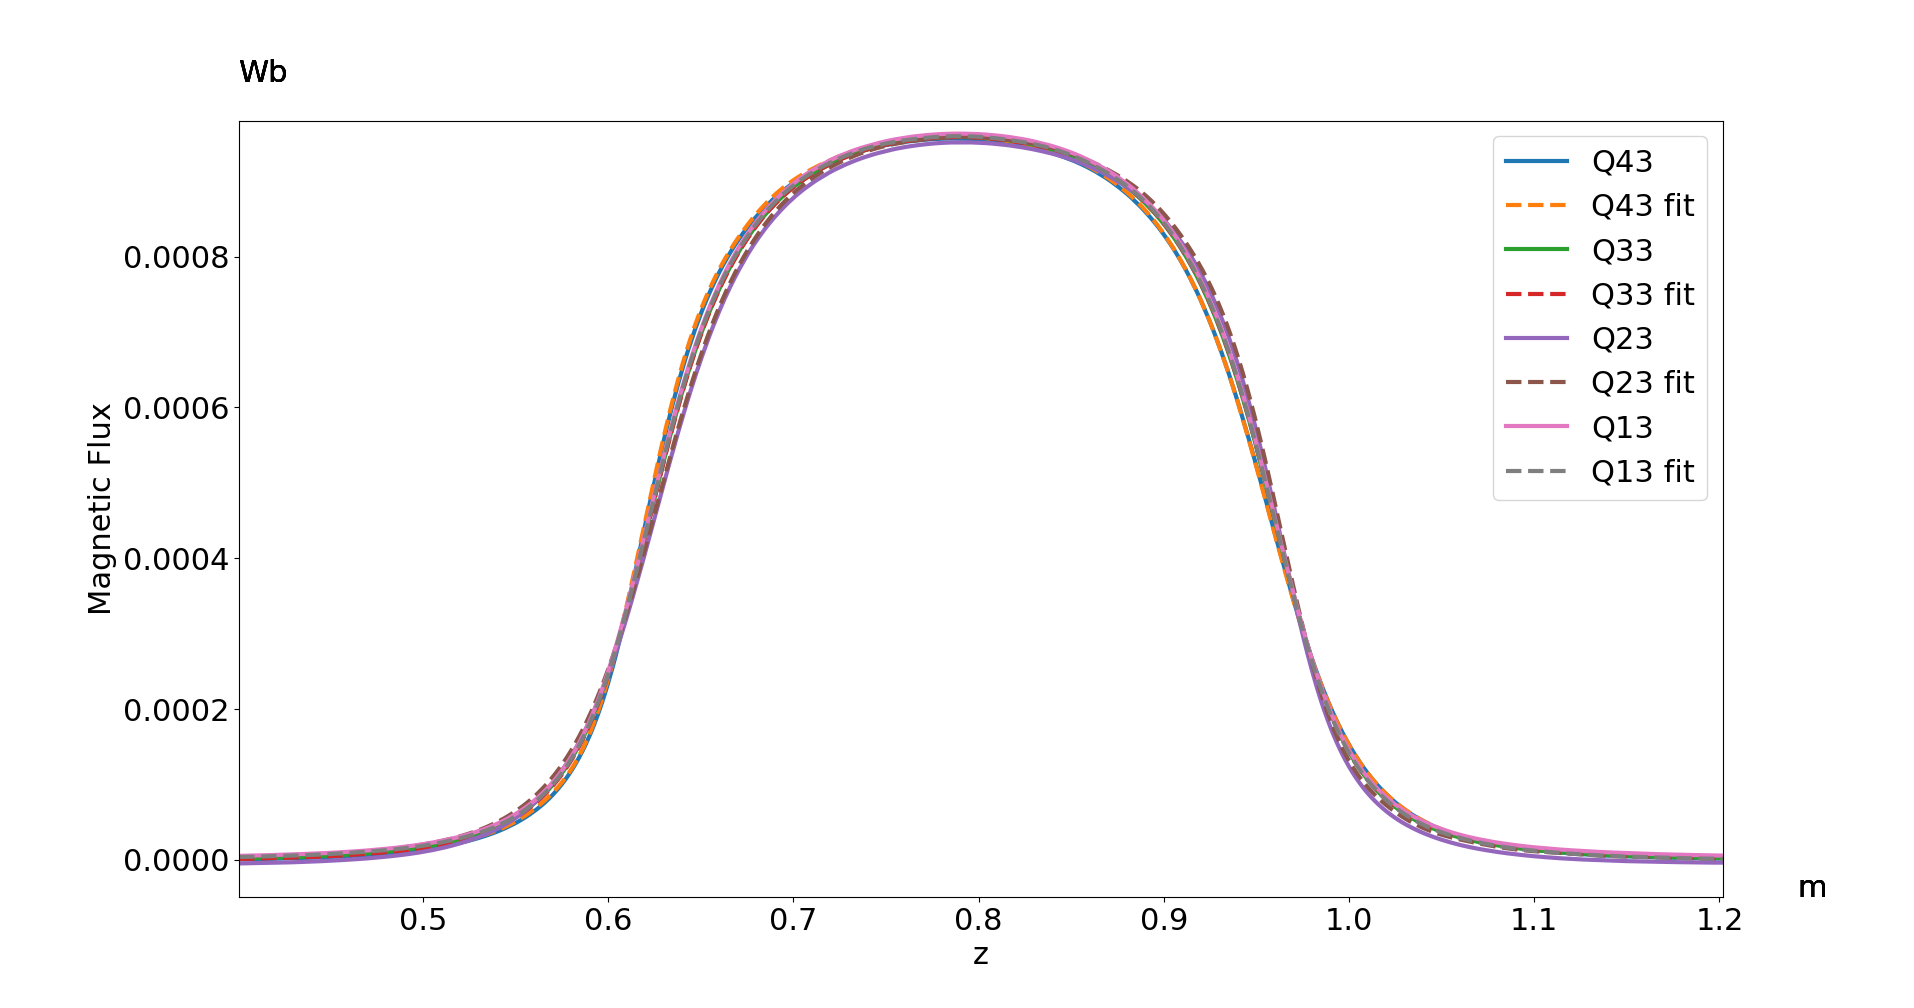
\includegraphics[width=\linewidth]{figs/Q3fit}
    \caption{Measurements and BFF fit, $Q_{q,3}$ coils.}
    \label{fig:Q3fit}
\end{figure}

\begin{figure}[!h]
    \centering
    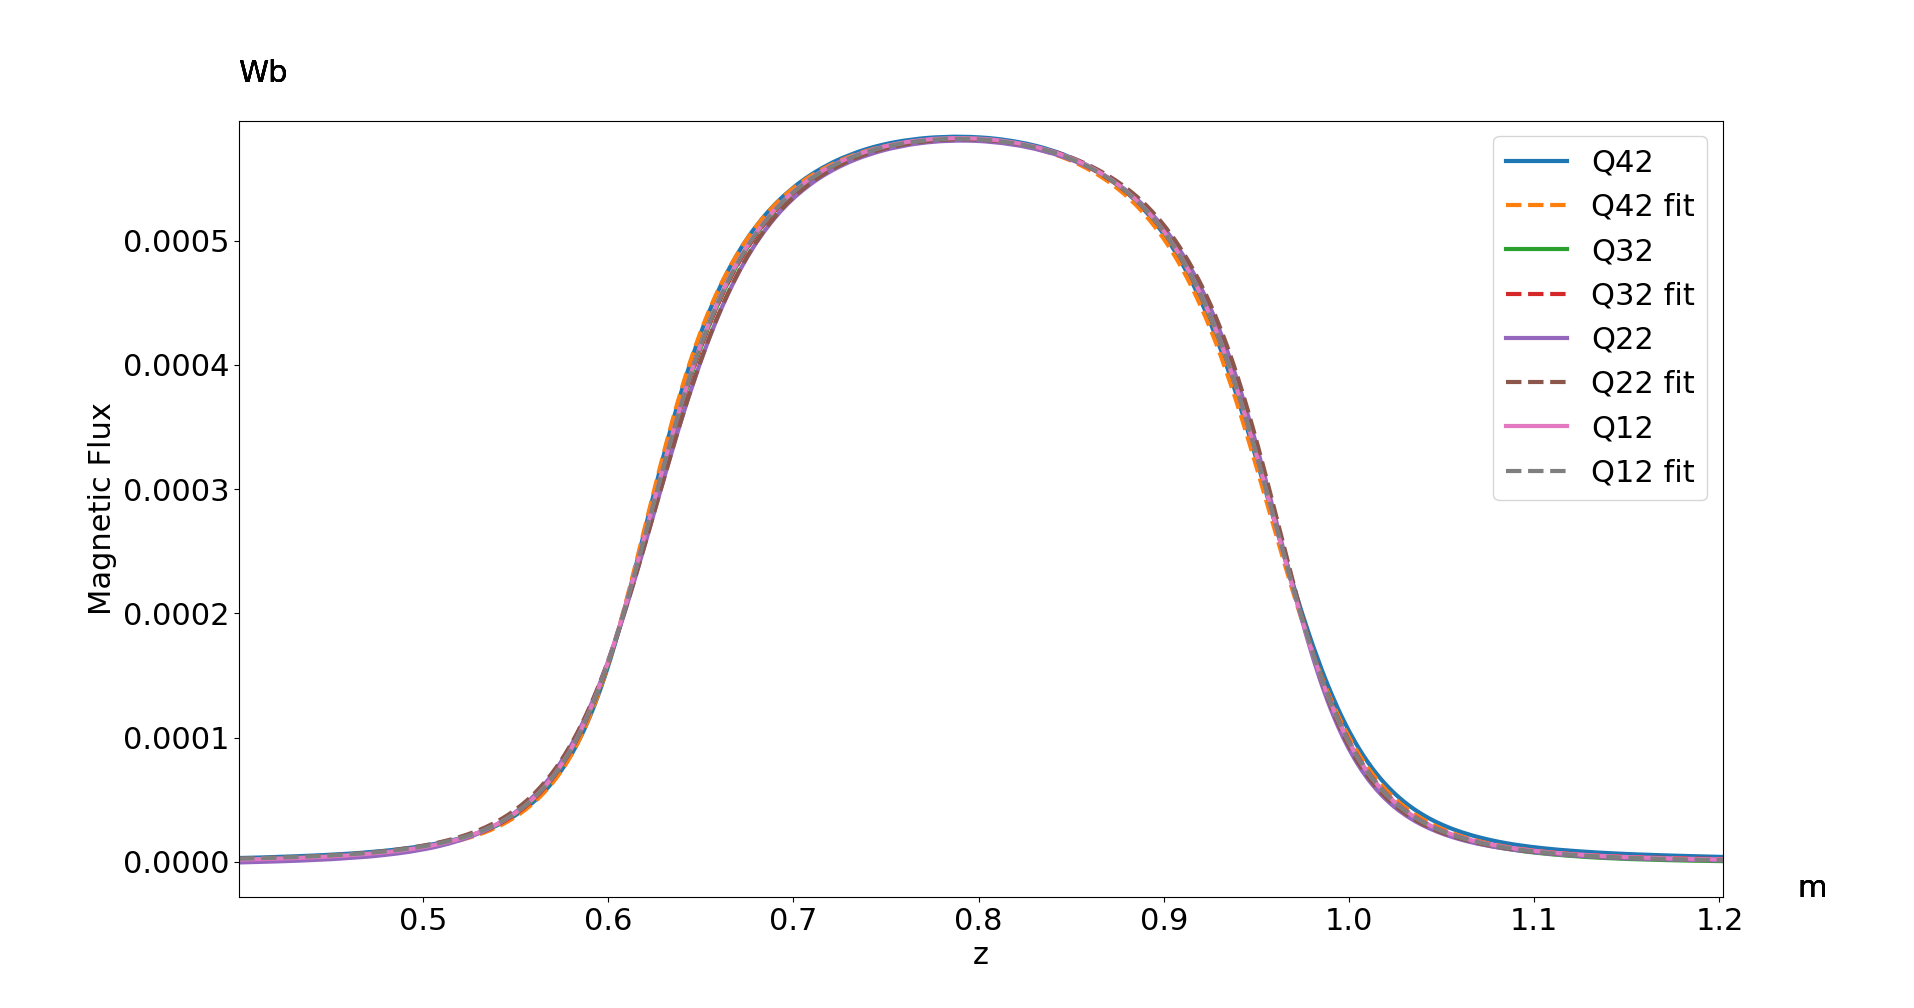
\includegraphics[width=\linewidth]{figs/Q2fit}
    \caption{Measurements and BFF fit, $Q_{q,2}$ coils.}
    \label{fig:Q2fit}
\end{figure}

\begin{figure}[!h]
    \centering
    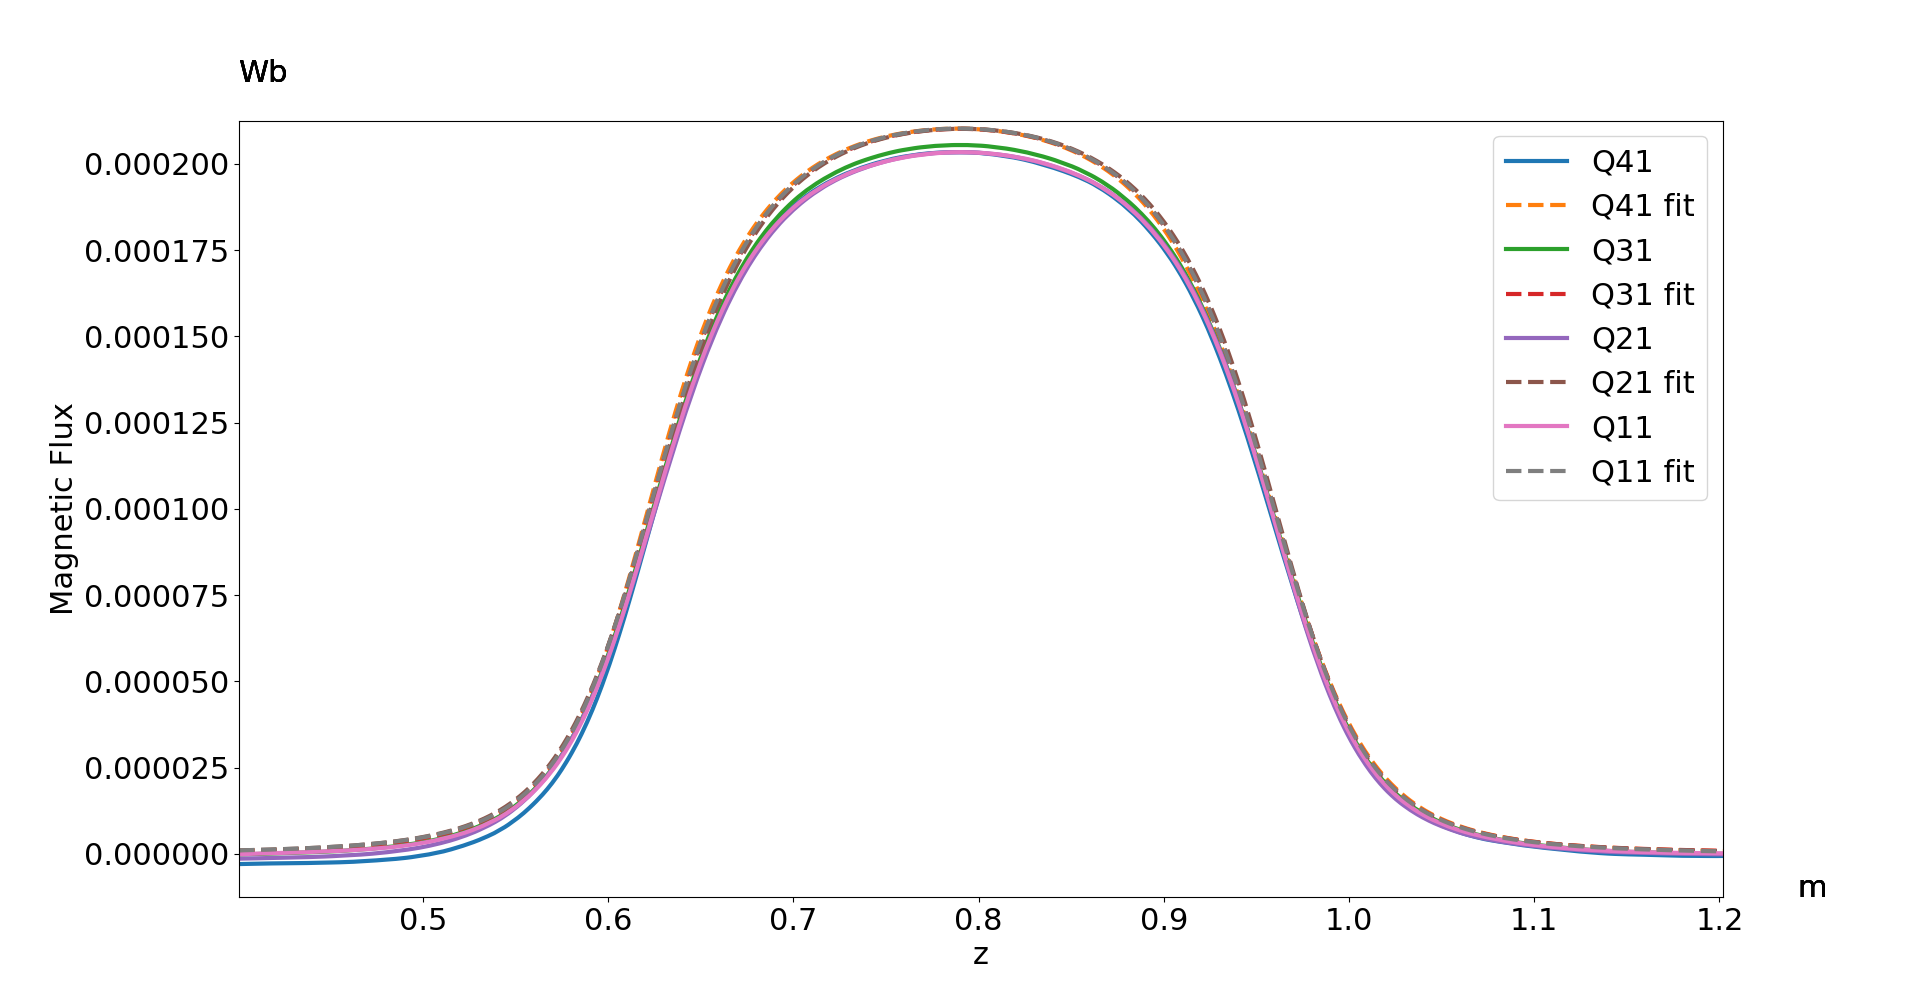
\includegraphics[width=\linewidth]{figs/Q1fit}
    \caption{Measurements and BFF fit, $Q_{q,1}$ coils.}
    \label{fig:Q1fit}
\end{figure}

\section{3D Field Maps}
With the measurements fitted, the now known $C_{n,k}$
coefficients can be used to estimate the $B_z$ field
anywhere inside the measurement domain. Some 3D maps
are presented in figures \ref{fig:3dmap}-\ref{fig:3dmapyz}

\begin{figure}[!h]
    \centering
    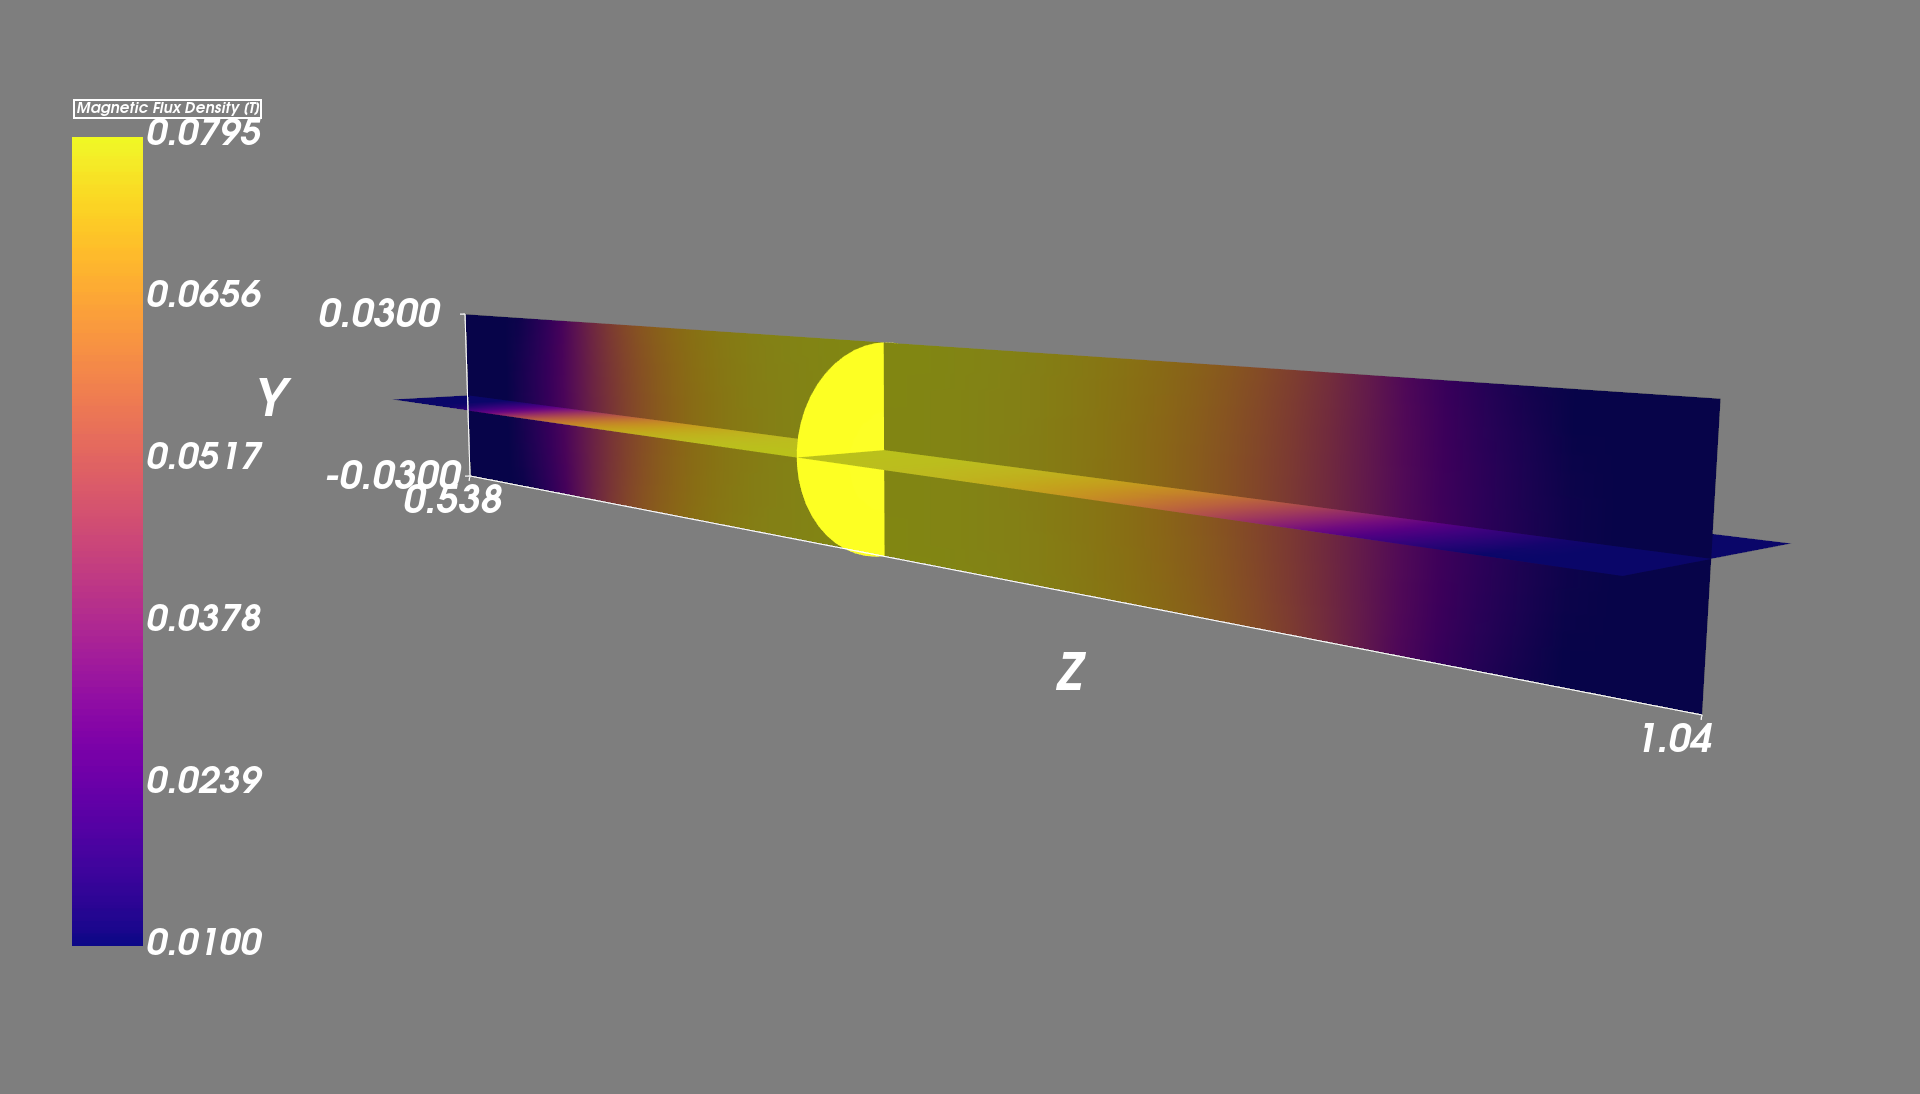
\includegraphics[width=\linewidth]{figs/3ddomain}
    \caption{3D field map of the estimated $B_z$ field.}
    \label{fig:3dmap}
\end{figure}

\begin{figure}[!h]
    \centering
    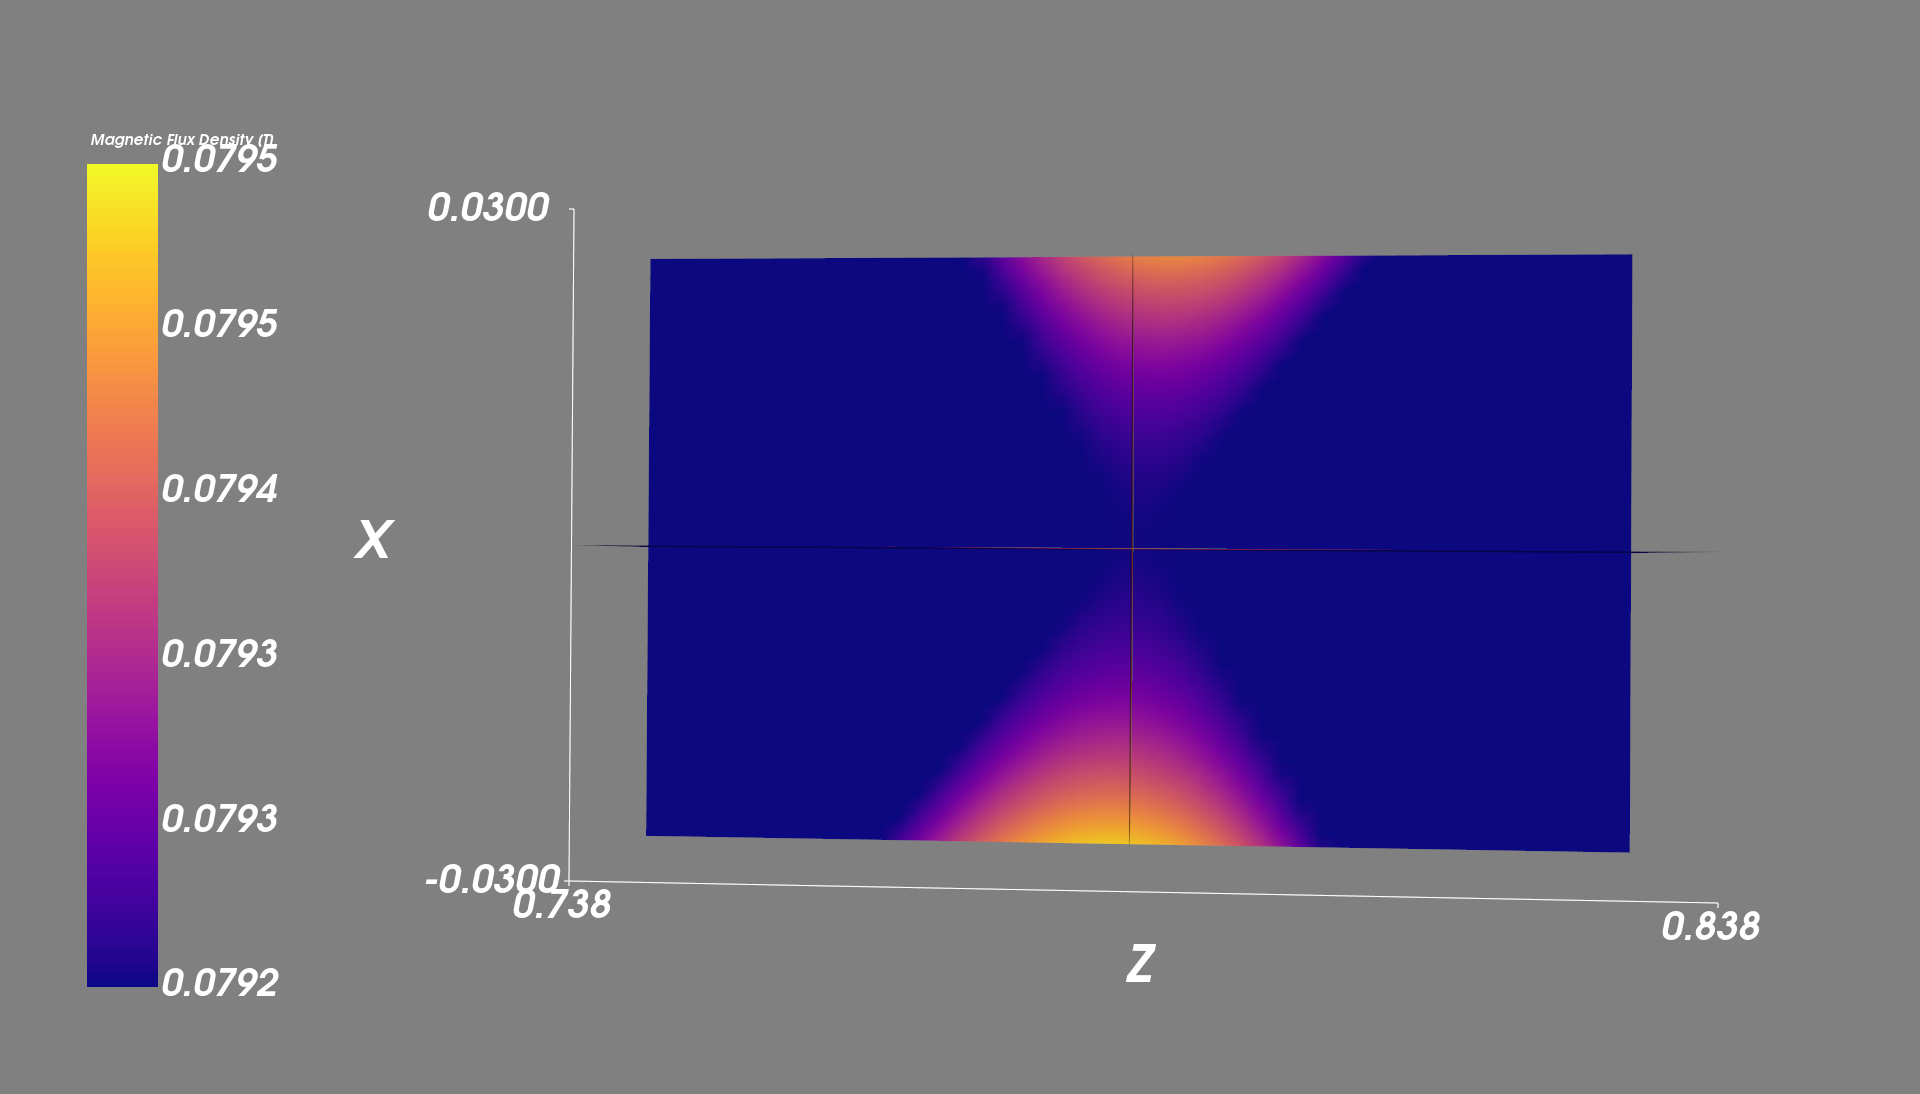
\includegraphics[width=\linewidth]{figs/3dxview}
    \caption{3D field map of the estimated $B_z$ field.
        $xz$ plane.}
    \label{fig:3dmapxz}
\end{figure}

\begin{figure}[!h]
    \centering
    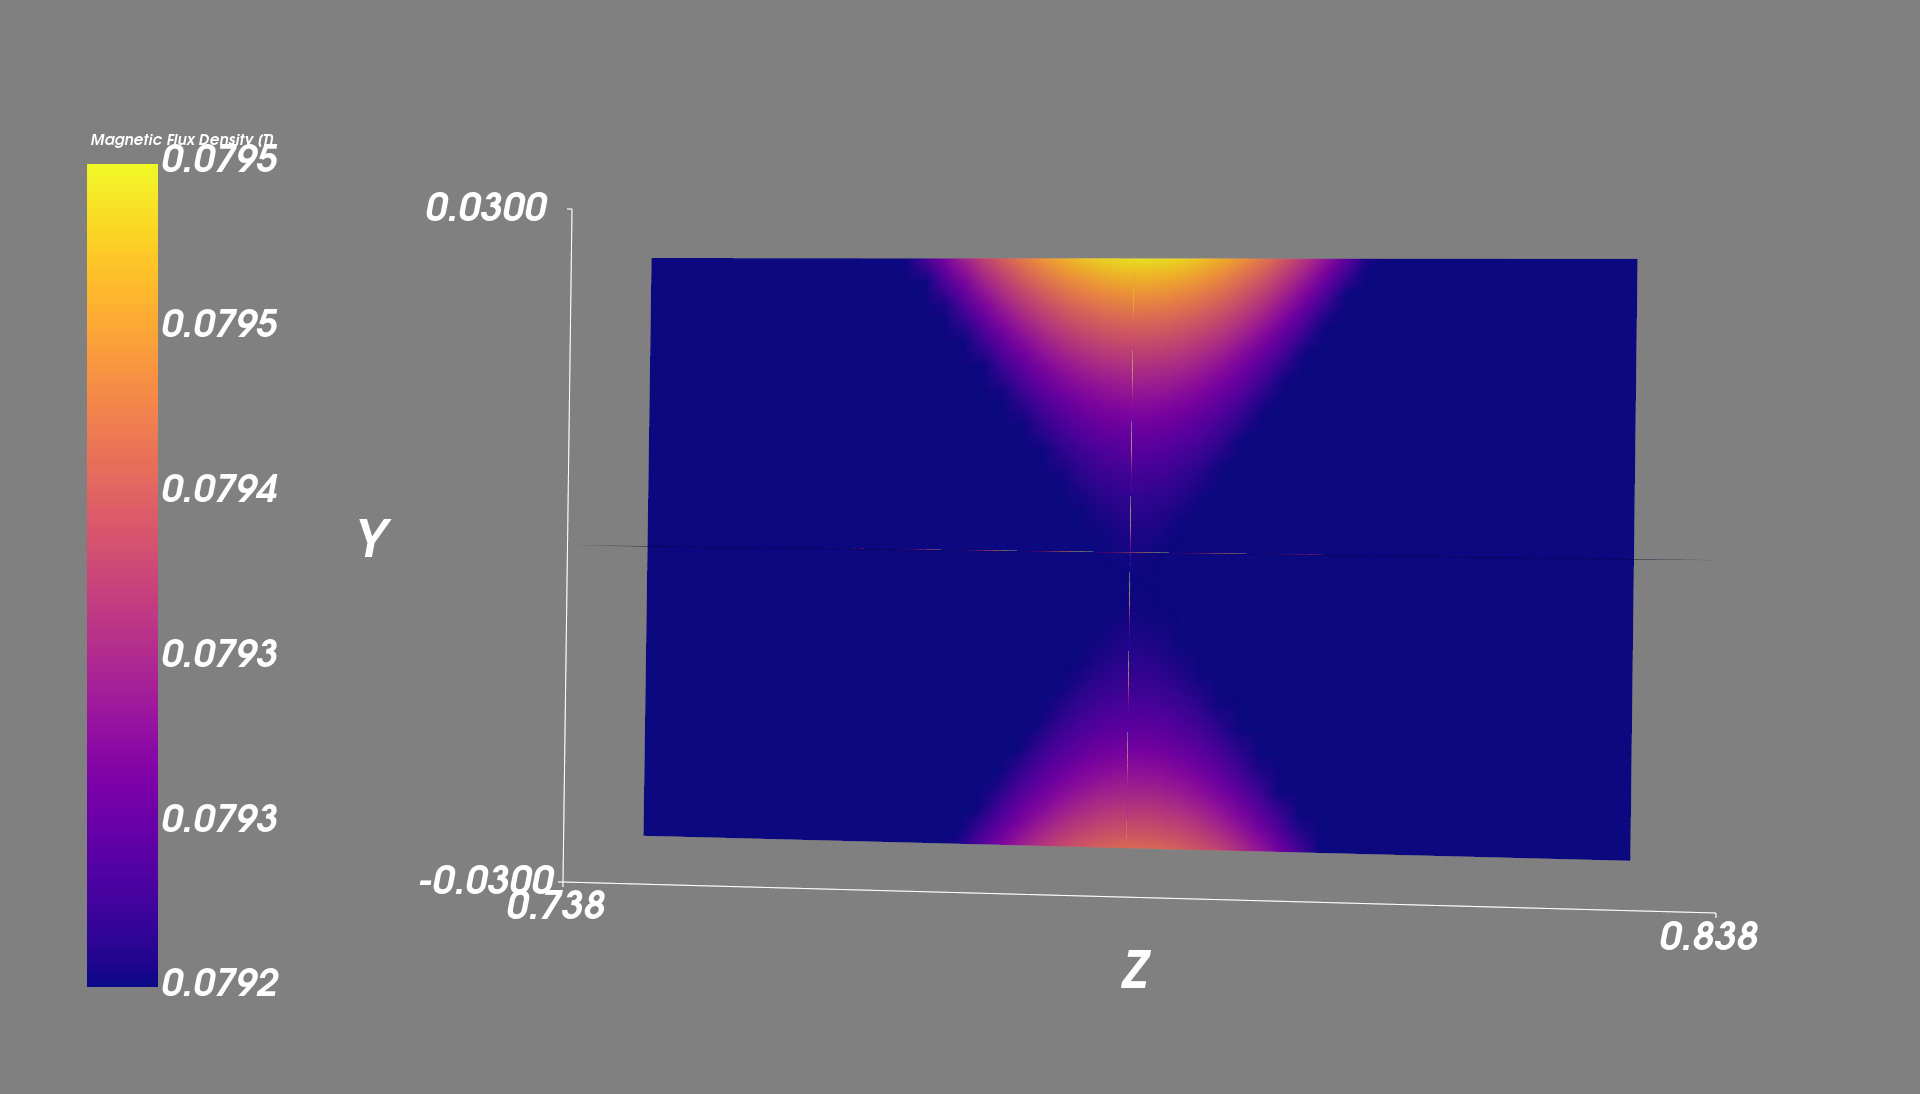
\includegraphics[width=\linewidth]{figs/3dyview.png}
    \caption{3D field map of the estimated $B_z$ field.
        $yz$ plane.}
    \label{fig:3dmapyz}
\end{figure}